\documentclass[border=5pt]{standalone}
\usepackage{tikz}
\usepackage{tikz-3dplot}
\usetikzlibrary{arrows.meta, 3d, perspective, calc}
\usepackage{amsmath}
\begin{document}
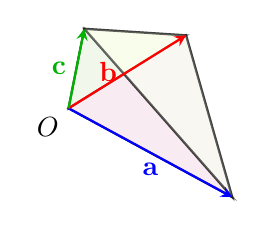
\begin{tikzpicture}[scale=0.8, >=stealth, 3d view={30}{70} ]
    % Define coordinates
    \coordinate (O) at (0,0,0);
    \coordinate (A) at (3,0,0);
    \coordinate (B) at (1,2,0);
    \coordinate (C) at (0,0.5,2.5);

    % Draw the tetrahedron
    \draw[thick, fill=blue!10, opacity=0.5] (O) -- (A) -- (B) -- cycle;
    \draw[thick, fill=red!10, opacity=0.5] (O) -- (A) -- (C) -- cycle;
    \draw[thick, fill=green!10, opacity=0.5] (O) -- (B) -- (C) -- cycle;
    \draw[thick, fill=yellow!10, opacity=0.5] (A) -- (B) -- (C) -- cycle;

    % Draw vectors
    \draw[->,thick,blue] (O) -- (A) node[midway,below] {$\mathbf{a}$};
    \draw[->,thick,red] (O) -- (B) node[midway,left] {$\mathbf{b}$};
    \draw[->,thick,green!70!black] (O) -- (C) node[midway,left] {$\mathbf{c}$};

    % Label vertices
    \node[below left] at (O) {$O$};
\end{tikzpicture}
\end{document}
